\subsection{Orchestrator}

This section describes the design of the \emph{Orchestrator}. The \emph{Orchestrator} is the
component that manages the task to be done in the cloud. It is running over the
\bonfire Cloud and controls all interactions between all the components implemented in \emph{Fed4FIRE} testbeds as \bonfire and \vw.
First, the \emph{Orchestrator}'s funcionalities and the interactions with other
components of the GEO-Cloud system are described. Then, the workflow of
\emph{Orchestrator} and the interfaces with the \emph{Archive and Catalog} module and the
\emph{Processing Chain} module are depicted.


\subsubsection{Functionality}

The \emph{Orchestrator} has the following functions:

\begin{itemize}
\item To identify which outputs shall be generated by the processors.
\item To generate the Job Orders. They contain all the necessary information
  that the processors need. Furthermore these \ac{XML} files include the interfaces and addresses of the folders in which the input information to the processors is located and the folders in which the outputs of the processors have to be sent. They also include the format in which the processors generate their output.
\item To look for raw data in the ground stations (pooling) to ingest such raw data in a shared storage unit in the cloud for its distribution to the processing chain.
\item To control the processing chain by communicating with the product processors, which have four levels of processing: L0, L1A, L1B and L1C.
\item To manage the archive and catalogue.
\end{itemize}

The orchestrator is designed to be implemented in the GEO-Cloud architecture. It
interacts with different modules:
\begin{itemize}

\item Ground stations implemented in \vw.
\item Processing instances in the cloud.
\item Archive and catalogue.
\end{itemize}

Figure~\ref{fig:orchestrator-interactions} depicts the \emph{Orchestrator’s} interactions with the other modules of the GEO-Cloud architecture.


\begin{figure}[!h]
\begin{center}
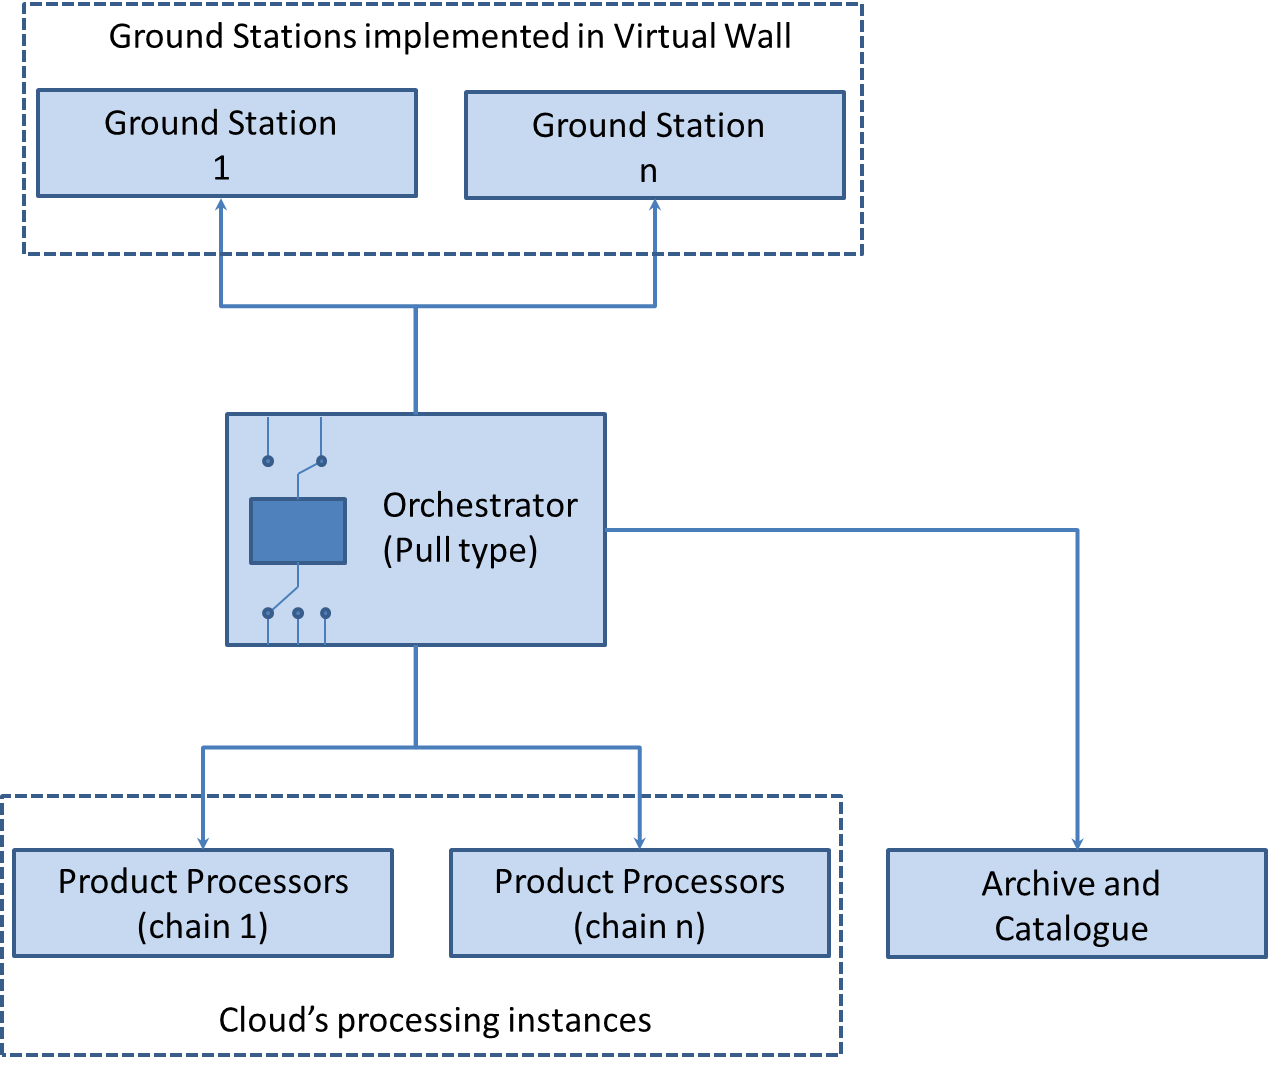
\includegraphics[width=0.5\textwidth]{cloud/orchestrator-interactions.png}
\caption{Orchestrator interactions}
\label{fig:orchestrator-interactions}
\end{center}
\end{figure}


As shown in Figure~\ref{fig:orchestrator-interactions}, the \emph{Orchestrator} is
pooling the Ground Stations frequently. When the \emph{Orchestrator} gets the data,
uses the Product Processor for processing the data to generate the result
image. When this processing has finished, the \emph{Orchestrator} sends the image to
Archive and Catalogue to be available for customers.

\subsubsection{Workflow}

The \emph{Orchestrator} works by following the next sequence of steps:
\begin{enumerate}
\item The \emph{Orchestrator} gets all the information about the \emph{Ground
    Stations Simulators} and localizes them.
\item The \emph{Listener} pools to the \emph{Ground Stations} and when there are
  a downloadable raw data, the \emph{New\_Data\_Event} is launched.
\item  When the \emph{New\_Data\_Event} occurs, the \emph{Orchestrator} downloads the data.
\item  The \emph{Orchestrator} moves the raw data to a shared storage.
\item Then, the \emph{Orchestrator} makes different \emph{Job Orders} for the processors. The \emph{Job Order} contains all the useful information for the \emph{Product Processors} to proceed with the image processing.
\item The \emph{Orchestrator} gets the \emph{ProcessorChainController} object (this object was made regarding \emph{Singleton pattern}).
\item The \emph{Orchestrator} instructs the \emph{ProcessorChainController} object to create a new processing chain by sending the \emph{JobOrders} created in step 4.
\item The \emph{ProcessorChain Controller} object creates a new \emph{Processing Chain} to process the data.
\item The \emph{Processing Chain} sequentially executes the L0, L1A, L1B, L1C processors.
\item When the \emph{ProcessingChain} has finished, this notifies the \emph{ProcessorChainController} object that the processing ended.
\item The \emph{ProcessingChainController} alerts the \emph{Orchestrator} that the \emph{Processing Chain} has finished.
\item The \emph{Orchestrator} takes the created image and puts it into the \emph{Archive}.
Figure~\ref{fig:orchestrator-workflow} depicts the workflow of the \emph{Orchestrator}.

\begin{figure}[!h]
\begin{center}
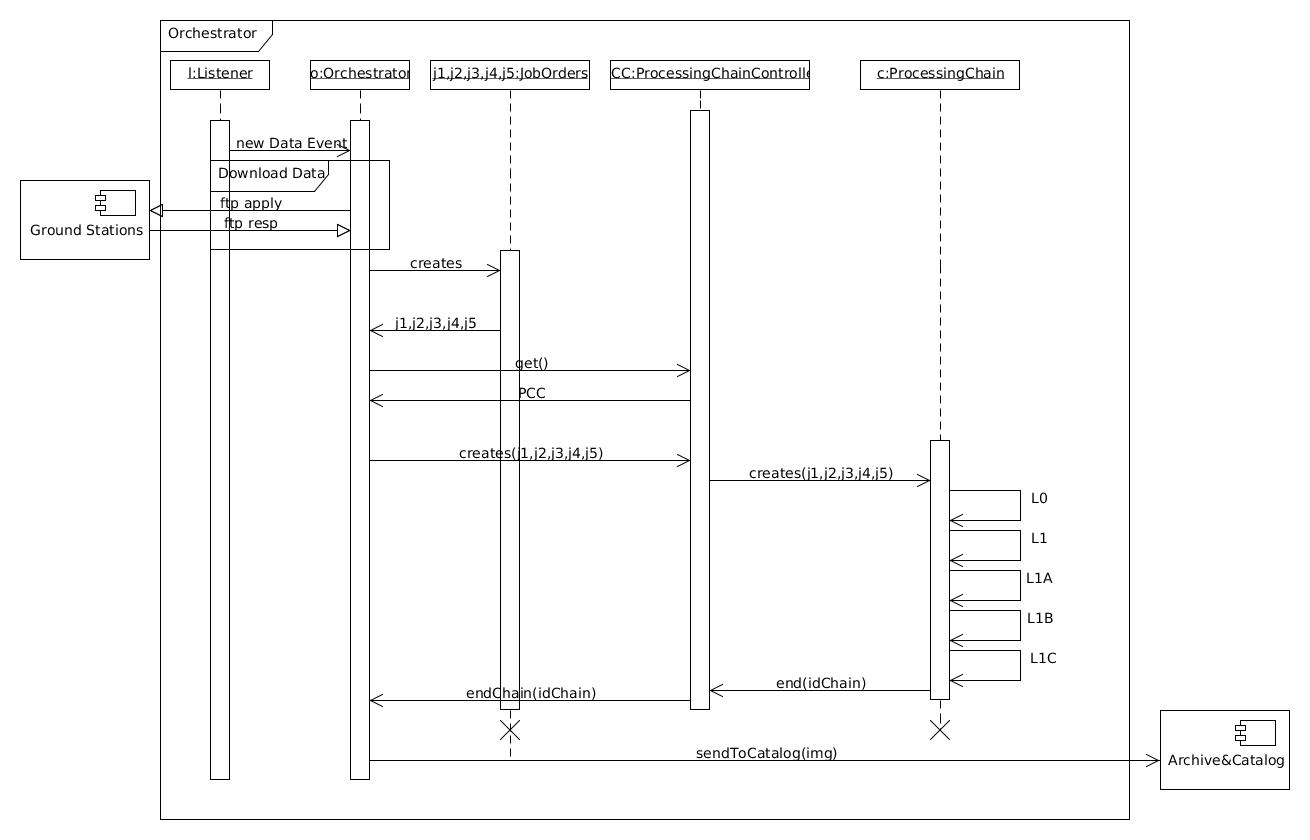
\includegraphics[width=1\textwidth]{cloud/orchestrator-workflow.jpg}
\caption{Orchestrator workflow}
\label{fig:orchestrator-workflow}
\end{center}
\end{figure}

\subsubsection{Interfaces}

The \emph{Orchestrator} has interfaces with the Ground Stations implemented in
\emph{Virtual Wall}, with the \emph{Product Processors} and with the
\emph{Archive and Catalogue}.
\paragraph{Interfaces with the Ground Stations implemented in Virtual Wall}~\\
The \emph{Ground Stations} are deployed in some \emph{Virtual Wall} nodes. In those, the impairments and features of the network are simulated. Essentially, the \emph{Orchestrator} is pooling those \emph{Ground Stations} over \ac{FTP} connections to know when a raw data is available. So, this Ground Stations are \ac{FTP} servers in which the \emph{Orchestrator} can get the raw data obtained by the constellation of satellites.
\paragraph{Interfaces with the Product Processors}~\\
The \emph{Orchestrator} communicates with the \emph{Product Processors} through the \emph{ProcessingChainController} instance as shown in Figure~\ref{fig:orchestrator-workflow}. The \emph{Orchestrator} commands the \emph{ProcessingChainController} to create a new processing chain to process the raw data. When this process finishes, the ProcessingChainController sends to the Orchestrator a message to indicate the end of the chain. Thus, the ProcessingChainController checks the product processors progress and initiates the next level until the processing chain finishes. Finally, the Orchestrator obtains the end product and locates it in the Catalogue Service. 

\subsubsection{Design}

\subsubsection{Implementation}

\subsubsection{Execution}

\subsubsection{Implementation in BonFIRE}




\subsection{Processing Chain}


The \emph{Processing Chain} is a module which is in charge of the processing of the
payload raw data from the satellites to produce image products. The four, most
important operations that the product processors perform on the input data are
the following:
\begin{itemize}
\item A calibration, to convert the pixel elements from instrument digital counts into radiance units.
\item A geometric correction, to eliminate distortions due to misalignments of the sensors in the focal plane geometry.
\item A geolocation, to compute the geodetic coordinates of the input pixels.
\item An ortho-rectification, to produce ortho-photos with vertical projection, free of distortions.
\end{itemize}

The previous steps also generate quality-related figures of merit that are made
available in all the products. Moreover, the product processors generate
metadata, in line with industry standards, to facilitate the cataloguing,
filtering and browsing of the product image collection. These processors are
considerated as black boxes because they are owned by Elecnor Deimos and their
design and implementation can not be published, but them were studied for
carrying out this project.

The output image products are classified into four different levels, according to the degree of processing that they have been subjected to (see Figure~\ref{fig:cloud-states-pp}):
\begin{itemize}

\item \emph{Level 0} products are unprocessed images, in digital count numbers.
\item \emph{Level L1A} products are calibrated products, in units of radiance.
\item \emph{Level L1B} products are calibrated and geometrically corrected products (ortho-rectified), blindly geolocated.
\item \emph{Level L1C} products are calibrated and geometrically corrected products (ortho-rectified), precisely geolocated using ground control points.
\end{itemize}

\begin{figure}[!h]
\begin{center}
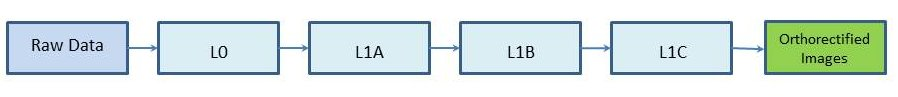
\includegraphics[width=0.8\textwidth]{detaildesign/stages-pp.jpg}
\caption{Stages of the product processing.}
\label{fig:cloud-states-pp}
\end{center}
\end{figure}

\subsubsection{The L0 Processor}

The acquired data is organized into image sectors of predefined size and structure and converted in scenes. Scenes, as defined here, are used throughout the subsequent L1 levels. The size and configuration of the scene is not changed again in the processing chain, for this reason the scene definition is constant for all the L1 levels.

The inputs are the following:
\begin{itemize}
\item The Raw Data.
\item The configuration database.
\item The calibration database.
\end{itemize}
The outputs are the following:
\begin{itemize}
\item The L0 products.
\end{itemize}

\subsubsection{The L1A Processor}

This section describes the functionality of the processors included in the Level 1A of the Automatic Processing Chain. The goal of Level 1A is to calibrate the scenes. The resulting images are given in units of radiances.

The L1A component works on the scenes that compound the L0 product, performing different transformations over pixel values to generate radiances.

The inputs to the L1A level are:
\begin{itemize}
\item One L0 scene.
\item The configuration database.
\item The calibration database.
\end{itemize}

The output is:
\begin{itemize}
\item The L1A product.
\end{itemize}

\subsubsection{The L1B Processor}
Level 1B implements the geolocation, resampling and packing.

The inputs to the L1B level are the following:
\begin{itemize}
\item The L1A product.
\item The configuration database.
\item The calibration database.
\end{itemize}

The outputs are the following:
\begin{itemize}
\item The L1B products.
\end{itemize}


\subsubsection{The L1C Processor}

The L1C processor performs the ortho-rectification of the L1B product using ground control points.

The inputs to the L1C level are the following:
\begin{itemize}
\item The L1B  product.
\item The calibration database.
\item The configuration database.
\end{itemize}

The output is the following:
\begin{itemize}
\item Orthorectified Images.
\end{itemize}

\subsubsection{Implementation in BonFIRE}




\subsection{Archive and Catalogue}


The \emph{Archive and Catalogue} is a shared space of memory between the \emph{Orchestrator}, the product processors and the distribution of data. It has a data acquisition component.

\emph{Data Acquisition component:} This component manages the input data arriving to the \emph{Archive and Catalog}. The ingestion of data is automatic.

In the \emph{Archive and Catalogue} module the processed images are stored and catalogued for their distribution.

The \emph{Archive and Catalogue} basically consists of:
\begin{itemize}
\item The \emph{Archive} is constituted by optimized storages structure allowing managing a big amount of data, efficient storage and retrieval of any kind of file. The \emph{Archive} shall be organized in hierarchical levels of storage in order to provide a cost effective storage solution.

\item The \emph{Catalogue} shall store an inventory database with the metadata of archive files. It allows the product process chain easiness to access to the metadata from the processed products.

\item For the added value services the catalog will be accessed by a \emph{Web Service}.

\item \ac{CSW} is a module with the \ac{CSW} standard for the catalogue (based on \ac{OGC} standard). For more information on \ac{CSW}, please refer to \ac{OGC} \emph{OpenGIS Implementation Specification 07-006r1} and the \ac{OGC} tutorial on \ac{CSW}. Through this standard the distribution of data is done.
\end{itemize}

\begin{figure}[!h]
\begin{center}
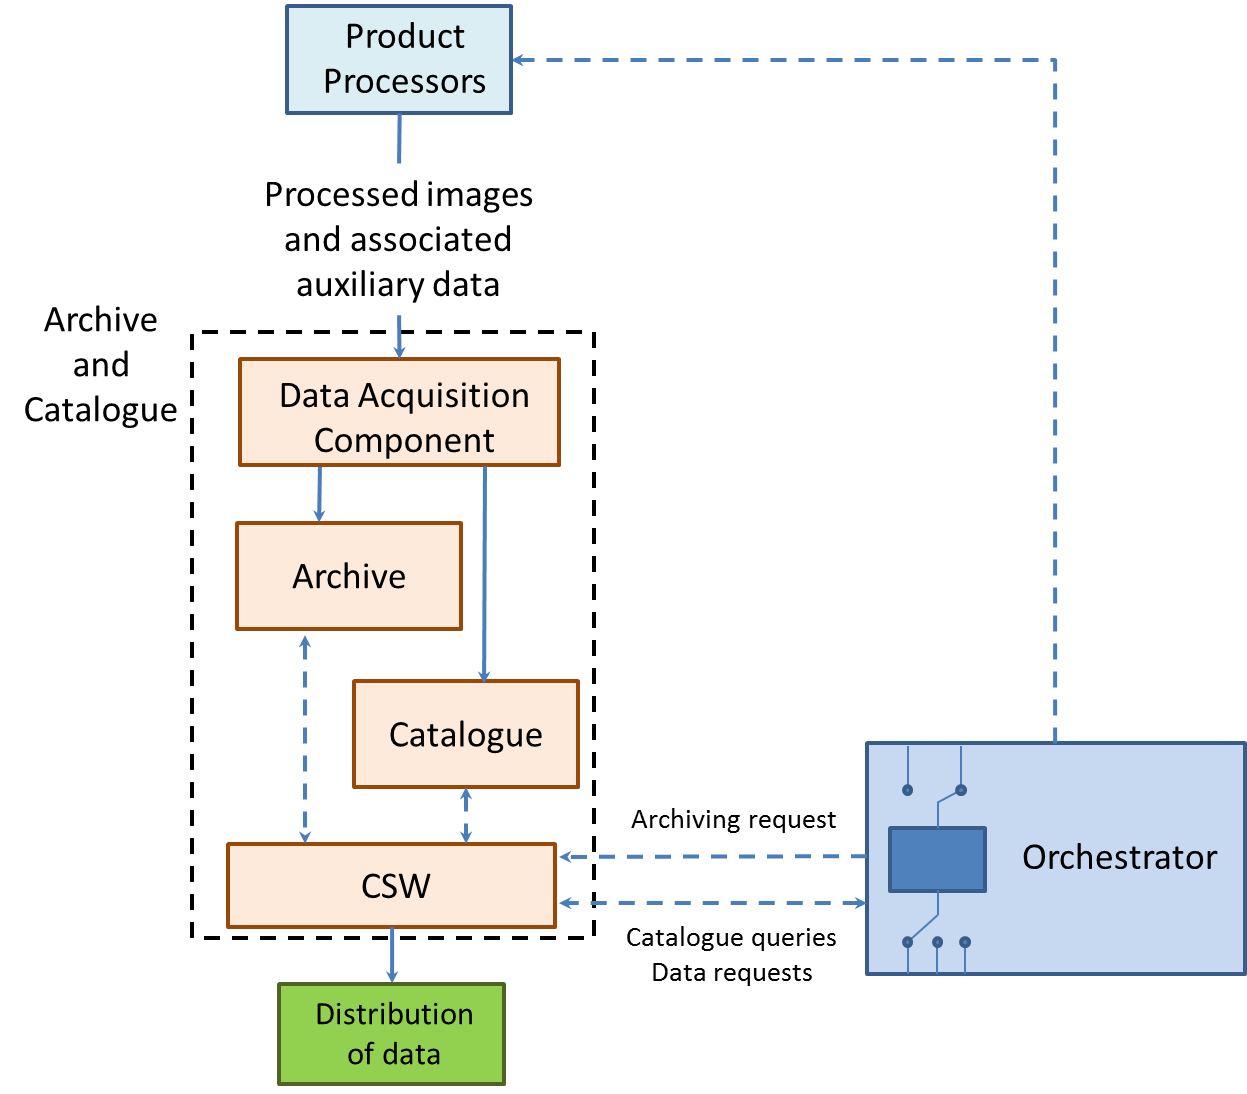
\includegraphics[width=0.6\textwidth]{detaildesign/scheme-archive-catalogue.png}
\caption{Scheme of the Archive and Catalogue module.}
\label{fig:archive-catalogue-scheme}
\end{center}
\end{figure}


\end{enumerate}


\subsubsection{Implementation}

\subsubsection{Execution}

\subsubsection{Implementation in BonFIRE}

